\section{Parallel Tractability of Datalog Programs}
\label{sec:ptclass}

Our target is to find for which kinds of ontologies (not ontology
languages) materialization is tractable in parallel. We consider
\emph{data complexity}, i.e., we \emph{assume that only the data is
  considered to be an input, whereas the rule set $R$ is fixed}.
  The data complexity of the materialization problem in this case
is $\texttt{PTime}$-complete, which is considered to be inherently
sequential in the worst case \cite{Raymond95}.
% Since we assume that, for any class of datalog programs where the rule
% set of each datalog program is fixed, the materialization problem is, thus, in data complexity
% $\texttt{PTime}$-complete, which is considered to be inherently sequential in the worst
% case \cite{Raymond95}.
In other words, the materialization problem of
datalog programs cannot be solved in parallel poly-logarithmic time unless \texttt{P}=\texttt{NC}.
Thus, we say that \emph{materialization for a class of datalog programs is tractable in parallel
if there exists an algorithm that handles this class of datalog programs and runs in parallel
poly-logarithmic time. Such an algorithm is also called an \texttt{NC} algorithm.}
In this section, we identify such classes of datalog programs by studying different \texttt{NC} algorithms.


\subsection{Parallel Tractability Classes}

We first give the following definition for a class of datalog programs
that is tractable in parallel, i.e., an \texttt{NC} algorithm exists
for handling each datalog program in this class.

\begin{definition}[Parallel Tractability Class]\label{def:ptd}
% Given a class $\mathcal{D}$ of
% datalog programs sharing the same rule set, we say that $\mathcal{D}$
% is a class of datalog programs with \emph{p}arallel
% \emph{t}ractability, short a \emph{\texttt{PTD} class},
% if there exists an \texttt{NC} algorithm that performs sound and complete materialization for each datalog program
% in $\mathcal{D}$. The corresponding class of ontologies of $\mathcal{D}$ is called a
% class of ontologies with parallel tractability, short a \texttt{PTO} class.

% \textcolor{red}{Suggested revision:} (Parallel Tractability Class).
  Let $R$ be a set of Datalog rules. Materialization w.r.t.\ to $R$ is
  tractable in parallel, if, for every set of facts $\textbf{I}$,
  there exists an \texttt{NC} algorithm that performs sound and
  complete materialization for $P=\langle R, \textbf{I}\rangle$; the
  set $\mathcal{D}$ of all such Datalog programs $P$ is called a
  \emph{\texttt{PTD} class}.  The corresponding class of ontologies of
  $\mathcal{D}$ is called a class of ontologies with parallel
  tractability, short a \texttt{PTO} class.
\end{definition}

According to the above definition, if we find an \texttt{NC} algorithm $\mathsf{A}$
for datalog materialization, then we can identify a \texttt{PTD} class $\mathcal{D}_{\mathsf{A}}$,
which is the class of all datalog programs that can be handled by $\mathsf{A}$.
However, current materialization algorithms of datalog rewritable ontology languages
(e.g., the core algorithm used in RDFox \cite{MotikNPHO14}) are not \texttt{NC} algorithms
due to their \texttt{PTime}-complete complexity, since they are
designed for handling general datalog programs. Thus, we proceed to
devise specific \texttt{NC} algorithms.
In the following, we first give a parallel materialization algorithm that works for
general datalog programs. We then restrict this algorithm to an \texttt{NC} version
and identify the target \texttt{PTD} class.


\subsection{Materialization Graph}

In order to give a parallel materialization algorithm,
we introduce the notion of \emph{materialization graphs}, which
facilitates the analysis of the given algorithm.

% \begin{definition}[Materialization Graph]\label{def:mg}
% A \emph{materialization graph}, with respect to
% a datalog program $P=\langle R, \textbf{I}\rangle$, is a directed acyclic graph
% denoted by $\mathcal{G}=\langle V, E\rangle$ where,
% \begin{enumerate}[leftmargin=4ex,label=$\bullet$]
%   \item $V$ is the node set and $V\subseteq T_R^{\omega}(\textbf{I})$;
%   \item $E$ is the edge set and $E\subseteq T_R^{\omega}(\textbf{I})\times T_R^{\omega}(\textbf{I})$.
% \end{enumerate}
% For each edge of the form $e(v_1, v_2)$ where $v_1$ and $v_2$ are two nodes,
% we say that the node $v_1$ is the parent (node) of $v_2$ and the node $v_2$ is the child (node)
% of $v_1$. Further, $\forall H,B_1,\ldots,B_n\in V$, $\mathcal{G}$ satisfies the following conditions:
% \begin{enumerate}[leftmargin=4ex,label=$\bullet$]
%   \item $H$ has a parent node or a child node;
%   \item if $H$ has an in-degree of $0$, then $H$ is an original fact of $P$;
%   \item $B_1,\ldots,B_n\rightarrow H\in P^*$ is satisfied if $e(B_1, H),\ldots,e(B_n, H)\in E$ and
%   $B_1,\ldots,B_n$ are all the parents of $H$.
% \end{enumerate}
% A materialization graph $\mathcal{G}$ is a \emph{complete materialization graph},
% when $\mathcal{G}$ contains all ground atoms in $T_R^{\omega}(\textbf{I})$.

% \textcolor{red}{Suggested revision:}
% (Materialization Graph).
% A \emph{materialization graph}, with respect to
% a datalog program $P=\langle R, \textbf{I}\rangle$, is a directed acyclic graph
% denoted by $\mathcal{G}=\langle V, E\rangle$ where,
% \begin{enumerate}[leftmargin=4ex,label=$\bullet$]
%   \item $V$ is the node set and $\textbf{I} \subseteq V\subseteq T_R^{\omega}(\textbf{I})$;
%   \item $E$ is the edge set and $E\subseteq T_R^{\omega}(\textbf{I})\times T_R^{\omega}(\textbf{I})$.
% \end{enumerate}
% For each edge of the form $e(v_1, v_2)$ where $v_1$ and $v_2$ are two nodes,
% we say that the node $v_1$ is the parent (node) of $v_2$ and the node $v_2$ is the child (node)
% of $v_1$. A materialization graph satisfies the following conditions:
% \begin{enumerate}[leftmargin=4ex,label=$\bullet$]
% \item each $v \in \textbf{I}$, $v$ has an in-degree of $0$;
% \item each $H \in V \setminus \textbf{I}$ such that $B_1,\ldots,B_n$
%   are all the parents of $H$, there is exactly one
%   $B_1,\ldots,B_n\rightarrow H\in P^*$.
% \end{enumerate}
% A materialization graph $\mathcal{G}$ is a \emph{complete materialization graph},
% when $\mathcal{G}$ contains all ground atoms in $T_R^{\omega}(\textbf{I})$.
% \end{definition}

\begin{definition}[Materialization Graph]\label{def:mg}
  A \emph{materialization graph} $\mathcal{G}$ with respect to a
  datalog program $P=\langle R, \textbf{I}\rangle$ is a directed
  acyclic graph $\langle V, E\rangle$ such that the set of nodes $V$
  satisfies $\textbf{I} \subseteq V\subseteq T_R^{\omega}(\textbf{I})$
  and the set of edges $E$ satisfies
  $E\subseteq T_R^{\omega}(\textbf{I})\times
  T_R^{\omega}(\textbf{I})$. For each edge $(v_1, v_2)$, we say that
  the node $v_1$ is the \emph{parent} (node) of $v_2$ and the node
  $v_2$ is the \emph{child} (node) of $v_1$. A materialization graph
  further satisfies the following conditions:
  \begin{itemize}
  \item each $v \in \textbf{I}$, $v$ has an in-degree of $0$;
  \item each $H \in V \setminus \textbf{I}$ such that $B_1,\ldots,B_n$
    are all the parents of $H$, there is exactly one
    $B_1,\ldots,B_n\rightarrow H\in P^*$.
  \end{itemize}
  A materialization graph $\mathcal{G}$ is a \emph{complete
    materialization graph} when $V$ contains all ground atoms in
  $T_R^{\omega}(\textbf{I})$.

  The \emph{size} of $\mathcal{G}$, denoted by $|\mathcal{G}|$, is the
  number of nodes in $\mathcal{G}$.  The depth of $\mathcal{G}$,
  denoted by \texttt{depth}($\mathcal{G}$), is the maximal length of a
  path in $\mathcal{G}$.
\end{definition}

For some derived atom $H$, there may exist several rule instantiations where $H$
occurs as a head atom.
This also means that $H$ can be derived in different ways.
The condition in the definition above results in only one way of deriving $H$ being
described by a materialization graph.
% Suppose $\mathcal{G}$ is a materialization graph such that the nodes
% with in-degree 0 are the
% original facts in $\textbf{I}$.
We next give an example of a materialization graph.\\

\begin{example}\label{exp:mg}
Consider a DHL($\circ$) ontology $\mathcal{O}_{\text{ex}_1}$ where the TBox is
$\{\exists R.A\sqsubseteq A\}$, the RBox is $\{S\circ R\sqsubseteq R\}$ and
the ABox is $\{A(b),R(a_1,b),S(a_i,a_{i-1})\}$ for $2\leq i\leq k$ and
$k$ an integer greater than $2$.
The corresponding datalog program of this ontology is $P_{\text{ex}_1}=\langle R, \textbf{I}\rangle$
where $\textbf{I}$ contains all the assertions in the ABox
and $R$ contains the two rules `$R(x,y),A(y)\rightarrow A(x)$'
and `$S(x,y),R(y,z)\rightarrow R(x,z)$'.
The graph in Figure~\ref{fig:mg} is a materialization graph with respect to $P_{\text{ex}_1}$,
denoted by $\mathcal{G}_{\text{ex}_1}$.
The nodes with in-degree 0 are the original facts in $\textbf{I}$;
each of the other nodes corresponds to a ground instantiation of some rule.
For example, the node $A(a_k)$ corresponds to the ground rule instantiation
`$R(a_k,b),A(b)\rightarrow A(a_k)$'.
The size of this materialization graph is the number of nodes, that is $3k$.
The depth of $\mathcal{G}_{\text{ex}_1}$ is $k$.
\end{example}

\begin{figure}[htbp]
\begin{center}
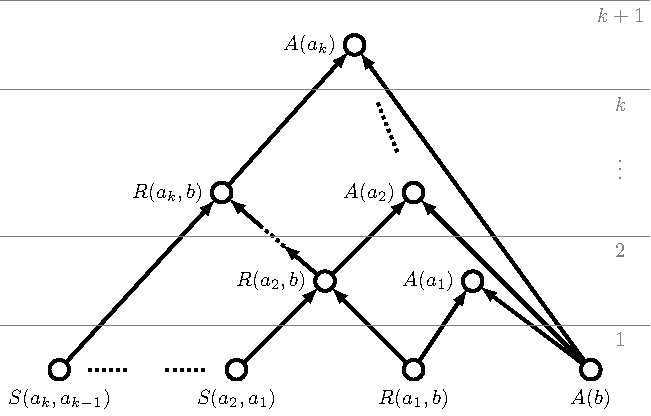
\includegraphics[width=0.7\textwidth]{fig-mg.pdf}
\caption{An example materialization graph}
\label{fig:mg}
\end{center}
\end{figure}

The set of nodes in a complete materialization graph is actually the result
of materialization.
Thus, the procedure of materialization can be transformed into the construction of
a complete materialization graph.
In the remainder, we only consider complete materialization graphs and
do not distinguish the term from the
notion of `materialization graphs'.
It should also be noted that there may exist several materialization graphs for a datalog program.


\subsection{A Basic Parallel Algorithm}
\label{sec:alg-bsc}

In this part, we propose a parallel algorithm
(denoted by Algorithm~$\mathsf{A}_{\text{bsc}}$) that constructs a materialization graph for a given datalog program.
Our computational model is a PRAM (parallel, random-access machine) that is mostly used to analyze parallel
complexity. This model allows us to introduce \emph{the parallel assumption}:
for any datalog program $P=\langle R, \textbf{I}\rangle$,
any substitution of some atom and any rule instantiation in $P^*$ can be mapped to a unique memory
location; further, a one-to-one relation can be established between processors and rule instantiations.
Under this assumption, a processor can check the applicability of its corresponding
rule instantiation and access the state of an atom occurring in this rule instantiation in constant time.
Algorithm~$\mathsf{A}_{\text{bsc}}$ is then given as follows.\\


\noindent\texttt{Algorithm~$\mathsf{A}_{\text{bsc}}$}. Given a datalog program $P=\langle R, \textbf{I}\rangle$,
the algorithm returns a materialization graph $\mathcal{G}$ of $P$.
Suppose we have $|P^*|$ processors, and each rule instantiation in $P^*$ is
assigned to one processor.
Initially $\mathcal{G}$ is empty. The following three steps are then performed:
\begin{enumerate}[leftmargin=8ex,label=(\textit{Step \arabic*}),ref=Step~\arabic*]
\item Add all facts in $\textbf{I}$ to $\mathcal{G}$.\label{alg1:addFacts}
\item For each rule instantiation $B_1,\ldots,B_n\rightarrow H$, if the body atoms are all
    in $\mathcal{G}$ while $H$ is not in $\mathcal{G}$,
    the corresponding processor adds $H$ to $\mathcal{G}$ and creates edges pointing
    from $B_1,\ldots,B_n$ to $H$.\label{alg1:updateG}
\item If no processor can add more nodes and edges to $\mathcal{G}$,
  terminate, otherwise continue with \ref{alg1:updateG}.\label{alg1:halt}\hfill$\Box$
\end{enumerate}

\begin{example}
We consider the datalog program $P_{\text{ex}_1}$ in Example~\ref{exp:mg} again,
and perform Algorithm~$\mathsf{A}_{\text{bsc}}$ on it.
Initially, all the facts ($A(b),R(a_1,b),S(a_2,a_1),\ldots,S(a_{k},a_{k-1})$) are added to the
result $\mathcal{G}_{\text{ex}_1}$ (\ref{alg1:addFacts}).
Then in different iterations of \ref{alg1:updateG}, the remaining nodes are added to
$\mathcal{G}_{\text{ex}_1}$ by different processors.
For example a processor $p$ is allocated a rule instantiation `$R(a_2,b),A(b)\rightarrow A(a_2)$'.
Then, processor $p$ adds $A(a_2)$ to $\mathcal{G}_{\text{ex}_1}$ after it checks that
$A(b)$ and $R(a_2,b)$ are in $\mathcal{G}_{\text{ex}_1}$.
Algorithm~$\mathsf{A}_{\text{bsc}}$ halts when $A(a_k)$ has been added to $\mathcal{G}_{\text{ex}_1}$ (\ref{alg1:halt}).
\end{example}

Lemma~\ref{lemma:a1} shows the correctness of Algorithm~$\mathsf{A}_{\text{bsc}}$ and that, for any datalog program $P$,
Algorithm~$\mathsf{A}_{\text{bsc}}$ always constructs a materialization graph with the minimum depth among all the
materialization graphs of $P$. The detailed proofs of Lemma~\ref{lemma:a1} and other lemmas and theorems can be found
in the appendix.

\begin{lemma}
\label{lemma:a1}
Given a datalog program $P=\langle R, \textbf{I}\rangle$, we have
\begin{enumerate}[leftmargin=4ex]
\item Algorithm~$\mathsf{A}_{\text{bsc}}$ halts and returns a materialization graph $\mathcal{G}$ of $P$;
\item $\mathcal{G}$ has the the minimum depth among all the materialization graphs of $P$.
\end{enumerate}
\end{lemma}

\begin{proof}[Proof sketch] This lemma can be proved by performing
an induction on $T_R^{\omega}(\textbf{I})$.
The stage (see the related contents in Section~\ref{sec:background}) of $P$
is the lower-bound of the depth of the materialization graphs. Based on the previous induction,
one can further check that, for the materialization graph $\mathcal{G}$ constructed by Algorithm~$\mathsf{A}_{\text{bsc}}$,
its depth is equal to the depth of the stage.
\end{proof}

We now discuss the parallel complexity of Algorithm~$\mathsf{A}_{\text{bsc}}$.
Given a class of datalog programs $\mathbb{P}$ where
a rule set is shared for each datalog program $P=\langle R, \textbf{I}\rangle$ in $\mathbb{P}$.
Let $e$, $v$ and $r$ represent the maximum arity of any predicate in $\textbf{I}$, the maximum number of variables
in any datalog rule, and the number of datalog rules respectively.
We then have that the number of
constants is at most $|\textbf{I}|e$, and the number of all possible rule instantiations in $P^*$
is at most $r(|\textbf{I}|e)^v$.
Note that $e, v$ and $r$ depend only on the rule set $R$ and not on the fact set $\textbf{I}$.
Thus, the memory space for storing the atoms and the rule instantiations is polynomial in the size of $\textbf{I}$.
This also means that the number of processors is polynomially bounded.
The computing time of \ref{alg1:addFacts} and \ref{alg1:halt} occupy constant time (denoted by $c_1$) because of parallelism.
Since Algorithm~$\mathsf{A}_{\text{bsc}}$ works under the parallel assumption, one iteration of
\ref{alg1:updateG} also costs constant time (denoted by $c_2$). Thus,
the whole computing time of Algorithm~$\mathsf{A}_{\text{bsc}}$ turns out to be $c_1+\ell\cdot c_2$
where $\ell$ denotes the number of iterations of \ref{alg1:updateG}.

An \texttt{NC} algorithm should meet two requirements: first,
it works on a polynomial number of processors; second, it halts in poly-logarithmic time.
As discussed above, Algorithm~$\mathsf{A}_{\text{bsc}}$ meets the first requirement.
If we want to restrict Algorithm~$\mathsf{A}_{\text{bsc}}$ to be an \texttt{NC} algorithm,
we can make the number of iterations of \ref{alg1:updateG} to be poly-logarithmically bounded.
We use the symbol $\psi$ to denote a poly-logarithmically bounded function.
For any datalog program, if we restrict the number of iterations of
\ref{alg1:updateG} to be bounded by $\psi(|\textbf{I}|)$,
the computing time of Algorithm~$\mathsf{A}_{\text{bsc}}$
is $c_1+\psi(|\textbf{I}|)\cdot c_2$. With this restriction, Algorithm~$\mathsf{A}_{\text{bsc}}$ is an \texttt{NC} algorithm denoted by
$\mathsf{A}_{\text{bsc}}^{\psi}$.

Based on $\mathsf{A}_{\text{bsc}}^{\psi}$, we can identify a class of datalog programs
$\mathcal{D}_{\mathsf{A}_{\text{bsc}}^{\psi}}$ such that all the datalog programs in it can be handled
by $\mathsf{A}_{\text{bsc}}^{\psi}$.
It is obvious that $\mathcal{D}_{\mathsf{A}_{\text{bsc}}^{\psi}}$ is a \texttt{PTD} class.
We use the following theorem to further show that this class can be captured based on
the materialization graphs of the datalog programs in $\mathcal{D}_{\mathsf{A}_{\text{bsc}}^{\psi}}$.

\begin{theorem}\label{theorem:a1}
For any datalog program $P=\langle R, \textbf{I}\rangle$, $P\in\mathcal{D}_{\mathsf{A}_{\text{bsc}}^{\psi}}$ iff $P$ has a
materialization graph whose depth is upper-bounded by $\psi(|\textbf{I}|)$.
\end{theorem}

\begin{proof}[Proof sketch]
We can first prove that the number of iterations
of \ref{alg1:updateG} is actually the depth of the constructed materialization
graph. This theorem then follows by considering
Lemma~\ref{lemma:a1}.
\end{proof}

Consider Example~\ref{exp:mg} again. Let the integer $k$ be a variable. We can
get a class of datalog programs, denoted by $\mathbb{P}_{\text{ex}_1}$, where the rule set
is $\{R(x,y),A(y)\rightarrow A(x), S(x,y),R(y,z)\rightarrow R(x,z)\}$ and the fact
set varies according to $k$. The algorithm $\mathsf{A}_{\text{bsc}}^{\psi}$ is restricted in the sense that it cannot even work on the rather simple datalog program class $\mathbb{P}_{\text{ex}_1}$.
Let $\mathcal{G}_{\text{ex}_1}$ be some materialization graph corresponding
to some datalog program in $\mathbb{P}_{\text{ex}_1}$. It can be checked that
\texttt{depth}($\mathcal{G}_{\text{ex}_1}$)$=k$ for some $k$.
This means that the depths of the materialization graphs are linearly bounded by $k$.
On the other hand, the sizes of the datalog programs in $\mathbb{P}_{\text{ex}_1}$ are polynomial in $k$.
Thus, for any $\psi$ that is poly-logarithmically bounded, we can always find a $k$ large
enough such that $\mathsf{A}_{\text{bsc}}^{\psi}$ terminates without constructing a materialization
graph for each datalog program in $\mathbb{P}_{\text{ex}_1}$.
However, there indeed exists an \texttt{NC} algorithm that can handle $\mathbb{P}_{\text{ex}_1}$.
We discuss this in the next part.


\subsection{Optimizing Algorithm~$\mathsf{A}_{\text{bsc}}$ via Single-Way Derivability}
\label{sec:opt}

In this part, we optimize Algorithm~$\mathsf{A}_{\text{bsc}}$ such that $P_{\text{ex}_1}$
can be handled. Based on the optimized variant of Algorithm~$\mathsf{A}_{\text{bsc}}$,
we can identify another \texttt{PTD} class.

We discuss our optimization based on a specific case in Example~\ref{exp:general}.
We find that, in this kind of case, the construction of a materialization graph can be accelerated.

\begin{figure}[htbp]
\begin{center}
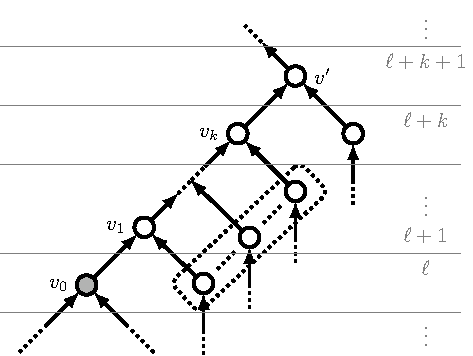
\includegraphics[width=0.6\textwidth]{fig-general.pdf}
\caption{A partial materialization graph}
\label{fig:general}
\end{center}
\end{figure}

\begin{example}\label{exp:general}
Consider the  snapshot of Algorithm~$\mathsf{A}_{\text{bsc}}$ in
Figure~\ref{fig:general}. A materialization graph $\mathcal{G}$
is being constructed for some datalog program $\langle R, \textbf{I}\rangle$.
The nodes in the dashed box denote the ones that have been added to $\mathcal{G}$.
In this snapshot, $v_0$ has been newly added
to $\mathcal{G}$ in the $\ell^{th}$ ($\ell\geq 1$) iteration.
Each of the nodes $v_i$ ($1\leq i\leq k$) has at most one parent node not in $\mathcal{G}$,
while $v'$ has two parent nodes not in $\mathcal{G}$.
All of the nodes $v_i$ ($1\leq i\leq k$) and $v'$ would be added to $\mathcal{G}$
afterwards.
\end{example}


In Example~\ref{exp:general}, $v_k$ would be added to $\mathcal{G}$ after \emph{at least} $k$
iterations by performing Algorithm~$\mathsf{A}_{\text{bsc}}$.
We can check that each edge $(v_{i-1},v_i)$ ($1\leq i\leq k$) in this
stage adheres to the condition:
\emph{if the parent node $v_{i-1}$ is derivable, the child node $v_i$ is derivable} (this
is because for a node $v_i$, the node $v_{i-1}$ is the only parent node that has not been added to $\mathcal{G}$).
We call this condition the \emph{single-way derivability condition}, which intuitively says that the derivability of a
node only depends on one of its parent nodes.
Observe that node $v_k$ is reachable from node $v_0$ through the path $\tau=(v_0,v_1,\ldots,v_k)$ where
each edge $(v_{i-1},v_i)$ ($1\leq i\leq k$) satisfies the single-way derivability condition.
We call such a path a \emph{single-way derivable} (SWD) path.
Further, the starting node $v_0$ in $\tau$ has been added to $\mathcal{G}$; in other words,
$v_0$ is derivable. Thus, all of the nodes $v_i$ ($1\leq i\leq k$) can be added to
$\mathcal{G}$ immediately.
Based on the above idea, we optimize Algorithm~$\mathsf{A}_{\text{bsc}}$ by checking whether such an SWD path
exits for some node $v$. If there is an SWD path for node $v$, this node can be added to $\mathcal{G}$
due to the single-way derivability condition.

For Example~\ref{exp:general},
there exists an SWD path $(v_0,\ldots,v_i)$ for each node $v_i$
($1\leq i\leq k$), hence, all of these nodes
can be added to $\mathcal{G}$ right after $v_0$. On the other hand,
node $v'$ has no SWD path since it has two parent nodes not in $\mathcal{G}$.

We next discuss how to determine the existence of SWD paths. Note that, SWD paths require us to
describe the reachability between two nodes. To this extent, we use a
binary transitive relation $\texttt{rch} \subseteq T_R^{\omega}(\textbf{I})\times T_R^{\omega}(\textbf{I})$,
e.g., \texttt{rch}$(v_1,v_2)$ means that $v_2$ is reachable from $v_1$.
In each iteration of \ref{alg1:updateG} in Algorithm~$\mathsf{A}_{\text{bsc}}$, we further compute as \texttt{rch}
relation (denoted by $S_{\textit{\!\tiny rch}}$) by performing the following process:

\begin{description}[leftmargin=4ex]
\item[(\textbf{\dag})] \emph{For each rule instantiation of the form $B_1,..,B_i,..,B_n\rightarrow H$
such that $H$ has not been added to $\mathcal{G}$}:
\begin{enumerate}[leftmargin=0ex]
\item \emph{if the all body atoms $B_1,\ldots,B_n$ have been added to $\mathcal{G}$, put \texttt{rch}$(B_1,H),\ldots,$ \texttt{rch}$(B_n,H)$ in $S_{\textit{\!\tiny rch}}$};
\item \emph{if $B_i$ is the only node in the body that has not been added to $\mathcal{G}$,
    put \texttt{rch}$(B_i,H)$ in $S_{\textit{\!\tiny rch}}$}.\hfill$\Box$
\end{enumerate}
\end{description}

We then compute the transitive closure (denoted by $S^*_{\!\textit{\tiny rch}}$) with respect to
$S_{\!\textit{\tiny rch}}$. Based on the transitive closure, we can
perform the following optimization:
for a node $v$, if there is a relation $\texttt{rch}(v',v)\in S^*_{\!\textit{\tiny rch}}$
such that $v'$ has been added to $\mathcal{G}$ and $v$ has an SWD
path, then $v$ can be added to $\mathcal{G}$.
The following algorithm applies this optimization strategy.\\

\noindent\texttt{Algorithm~$\mathsf{OPT}$}. The algorithm requires two inputs:
a datalog program $P=\langle R, \textbf{I}\rangle$ and a (partial) materialization graph $\mathcal{G}$ that is
being constructed from $P$. The following steps are performed:
\begin{enumerate}[leftmargin=6ex,label=(\textbf{\roman*})]
\item Compute the \texttt{rch} relation $S_{\!\textit{\tiny rch}}$ by following the above process (see $(\textbf{\dag})$).\label{rch}
\item Compute the transitive closure $S^*_{\!\textit{\tiny rch}}$ of $S_{\!\textit{\tiny rch}}$.\label{transClos}
\item Update $\mathcal{G}$ as follows: for any \texttt{rch}$(B_i,H)\in S_{\!\textit{\tiny rch}}$
that corresponds to `$B_1,..,B_i,..$ $,B_n\rightarrow H$'
    and there exists a node $B'$ such that \texttt{rch}$(B',B_i)\in S^*_{\!\textit{\tiny rch}}$ and $B'$ is
    in $\mathcal{G}$; if $H$ is not in $\mathcal{G}$ or $H$ is in $\mathcal{G}$ but has no parent pointing
    to it, add $H$ and $B_i$ (if $B_i$ is not in $\mathcal{G}$) to $\mathcal{G}$, and create the edges
    $e(B_1, H), \ldots, e(B_n, H)$ in $\mathcal{G}$. Do nothing for other statements
    \texttt{rch}$(B_j,H)\in S_{\!\textit{\tiny rch}}$.\label{updateG}\hfill$\Box$
\end{enumerate}

It is well known that there is an \texttt{NC} algorithm for computing the
transitive closure \cite{Allender07}.
Based on this result and Algorithm~$\mathsf{OPT}$, we propose an optimized variant of Algorithm~$\mathsf{A}_{\text{bsc}}$:\\

\noindent\texttt{Algorithm~$\mathsf{A}_{\text{opt}}$}. Given a datalog program $P=\langle R, \textbf{I}\rangle$, the algorithm
returns a materialization graph $\mathcal{G}$ of $P$.
Suppose we have $|P^*|$ processors, and each rule instantiation in $P^*$ is
assigned to one processor.
Initially $\mathcal{G}$ is empty. The following steps are then performed:
\begin{enumerate}[leftmargin=8ex,label=(\textit{Step \arabic*}),ref=Step~\arabic*]
\item Add all facts in $\textbf{I}$ to $\mathcal{G}$.\label{alg3:addFacts}
\item Compute $S_{\!\textit{\tiny rch}}$ by performing \ref{rch} in Algorithm~$\mathsf{OPT}$; use an \texttt{NC}
    algorithm to compute the transitive closure $S^*_{\!\textit{\tiny rch}}$ (see \ref{transClos} in Algorithm~$\mathsf{OPT}$);
    update $\mathcal{G}$ by performing \ref{updateG}  in Algorithm~$\mathsf{OPT}$.\label{alg3:updateG}
\item If no node has been added to $\mathcal{G}$ (in \ref{alg3:updateG}), terminate,
    otherwise iterate \ref{alg3:updateG}. \label{alg3:halt}\hfill$\Box$
\end{enumerate}

It should be noted that there has to be an SWD path for any derivable node in some iteration when performing
Algorithm~$\mathsf{A}_{\text{opt}}$.
The following lemma shows the correctness of Algorithm~$\mathsf{A}_{\text{opt}}$.

\begin{lemma}\label{lemma:a3}
Given a datalog program $P=\langle R, \textbf{I}\rangle$,
$\mathsf{A}_{\text{opt}}$ halts and outputs a materialization graph $\mathcal{G}$ of $P$.
\end{lemma}

\begin{example}\label{exp:opt}
We perform Algorithm~$\mathsf{A}_{\text{opt}}$ on the datalog program $P_{\text{ex}_1}$ in Example~\ref{exp:mg}.
Initially, $R(a_1,b)$ is in the materialization graph $\mathcal{G}_{\text{ex}_1}$.
In the first iteration of \ref{alg3:updateG}, all the rule instantiations are in two kinds of forms:
`$R(a_i,b),A(b)\rightarrow A(a_i)$' and `$S(a_i,a_{i-1}),$ $R(a_{i-1},b)\rightarrow R(a_i,b)$', $2\leq i\leq k$,
$S_{\!\textit{\tiny rch}}$ is the set $\{$\texttt{rch}$(R(a_{i-1},b),
R(a_i,b)) \mid 2\leq i\leq k\}
\cup\{$\texttt{rch}$(R(a_i,b), A(a_i)) \mid 1\leq i\leq k\}$.
In the transitive closure of $S_{\!\textit{\tiny rch}}$,
one can check that \texttt{rch}$(R(a_1,b), R(a_i,b)),$
\texttt{rch}$(R(a_1,b), A(a_i))\in S^*_{\!\textit{\tiny rch}}, 2\leq i\leq k$.
Thus, $R(a_i,b)$ and $A(a_i)$, $2\leq i\leq k$, can all be added to
$\mathcal{G}_{\text{ex}_1}$
in the first iteration of \ref{alg3:updateG}.
\end{example}

We now analyse the parallel complexity of Algorithm~$\mathsf{A}_{\text{opt}}$.
We use the same symbols $e$, $v$ and $r$ that are used for analyzing the complexity of Algorithm~$\mathsf{A}_{\text{bsc}}$
(see Section~\ref{sec:alg-bsc}). Similarly to the analysis for Algorithm~$\mathsf{A}_{\text{bsc}}$, it can be checked that
the number of processors is polynomial in $|\textbf{I}|$, i.e., $r(|\textbf{I}|e)^v$.
We now consider the computing time of Algorithm~$\mathsf{A}_{\text{opt}}$. It
is obvious that \ref{alg3:addFacts} and
\ref{alg3:halt} occupy constant time (denoted by $c_1$). In \ref{alg3:updateG}, the phases of
computing $S_{\!\textit{\tiny rch}}$ and updating $\mathcal{G}$ also take constant time (denoted by $c_2$)
under the parallel assumption. Recall that the number of constants is at most $|\textbf{I}|e$ (see Section~\ref{sec:alg-bsc}).
Let $w$ and $p$ represent the maximum arity of any predicate and the number of predicates, respectively.
We have that the number of all possible substitutions of atoms is at most $p(|\textbf{I}|e)^w$.
The relation $S_{\!\textit{\tiny rch}}$ consists of pairs of the atoms. Thus, the size of $S_{\!\textit{\tiny rch}}$
is bounded by $p^2(|\textbf{I}|e)^{2w}$. It can be checked that the computing time of the \texttt{NC} algorithm for computing the transitive
closure of $S_{\!\textit{\tiny rch}}$ is poly-logarithmic in the size of $\textbf{I}$, more precisely,
it is upper bounded by $\log^2(p^2(|\textbf{I}|e)^{2w})$ ($=4\log^2(p)+4w^2\log^2(|\textbf{I}|e)+8w\log(p)\log(|\textbf{I}|e)$).
We now have that the total computing time of
Algorithm~$\mathsf{A}_{\text{opt}}$ is $c_1+\ell c_3 + \ell
c_4\log(|\textbf{I}|e) +\ell c_5\log^2(|\textbf{I}|e)$
where $c_3=c_2+4\log^2(p)$, $c_4=8w\log(p)$, $c_5=4w^2$ and $\ell$ denotes the number of iterations of \ref{alg3:updateG}.

Algorithm~$\mathsf{A}_{\text{opt}}$ can be restricted to an \texttt{NC} algorithm analogously to the process
for Algorithm~$\mathsf{A}_{\text{bsc}}$. That is the number of iterations of \ref{alg3:updateG}
is poly-logarithmically bounded, i.e., it is bounded by $\psi(|\textbf{I}|)$
where $\psi$ is a poly-logarithmic function. In this way, the computing time of
Algorithm~$\mathsf{A}_{\text{bsc}}$ turns out to be $c_1+c_3\psi(|\textbf{I}|)+c_4\psi(|\textbf{I}|)\log(|\textbf{I}|e)+
c_5\psi(|\textbf{I}|)\log^2(|\textbf{I}|e)$,
which is still poly-logarithmical in the size of $\textbf{I}$. We denote the
\texttt{NC} variant of Algorithm~$\mathsf{A}_{\text{opt}}$ by $\mathsf{A}_{\text{opt}}^{\psi}$.

Based on $\mathsf{A}_{\text{opt}}^{\psi}$, we can identify a \texttt{PTD} class $\mathcal{D}_{\mathsf{A}_{\text{opt}}^{\psi}}$.
Further, we have the following corollary, which implies that $\mathsf{A}_{\text{opt}}^{\psi}$ performs better
than $\mathsf{A}_{\text{bsc}}^{\psi}$ in terms of computing time.

\begin{corollary}
For any poly-logarithmically bounded function $\psi$,
we have that $\mathcal{D}_{\mathsf{A}_{\text{bsc}}^{\psi}}\subseteq\mathcal{D}_{\mathsf{A}_{\text{opt}}^{\psi}}$.
\end{corollary}

\begin{proof}[Proof sketch]
Suppose $P=\langle R,\textbf{I}\rangle\in\mathcal{D}_{\mathsf{A}_{\text{bsc}}^{\psi}}$. According to Theorem~\ref{theorem:a1},
the depth of the materialization graph $\mathcal{G}$ constructed by $\mathsf{A}_{\text{bsc}}^{\psi}$ is
upper-bounded by $\psi(|\textbf{I}|)$.
It is obvious that the number of nodes in each path of $\mathcal{G}$ is also upper-bounded by $\psi(|\textbf{I}|)$.
According to the optimization strategy applied in $\mathsf{A}_{\text{opt}}$, if $\mathcal{G}$ can be constructed
by $\mathsf{A}_{\text{opt}}$, the number of iterations of $\mathsf{A}_{\text{opt}}$ has to be upper-bounded by $\psi(|\textbf{I}|)$;
if $\mathcal{G}$ is not the materialization graph constructed
by $\mathsf{A}_{\text{opt}}$, then there has to exist another materialization graph $\mathcal{G}'$ constructed by $\mathsf{A}_{\text{opt}}$
and $\mathcal{G}'$ has a smaller depth compared to $\mathcal{G}$.
\end{proof}



%%% Local Variables:
%%% mode: latex
%%% TeX-master: "parallel-tractability-J"
%%% End:
